\documentclass [11pt,twoside]{article}
\usepackage[utf8]{inputenc}
\usepackage[T1]{fontenc}

%Page margins, header and footer positions
\usepackage{geometry}
 \geometry{
 a4paper,
 total={210mm,297mm},
 left=25mm,
 right=25mm,
 top=30mm,
 bottom=25mm,
 headsep=7mm}

\interfootnotelinepenalty=10000

%To display filling dots in the TOC for all entries
\usepackage[titles]{tocloft}
\renewcommand{\cftsecleader}{\cftdotfill{\cftdotsep}}

%Define new header and footer style
\usepackage{fancyhdr}

\pagestyle{fancy}
\fancyhf{}
\lhead{\color{Gray}{\small{DREAM - Marra, Miceli, Mora}}}
\lfoot{\textcolor{Gray}{\small{Copyright © 2021, Marra, Miceli, Mora – All rights reserved}}}
\rfoot{\textcolor{Gray}{\thepage}}
\renewcommand{\headrulewidth}{0pt}

%PACKAGES
\usepackage{wasysym}
\usepackage{pifont}
\usepackage{color, colortbl}
\definecolor{Gray}{gray}{0.9}

\newcommand{\supported}{\ding{52}\xspace}
\newcommand{\unsupported}{\ding{55}\xspace}
\newcommand{\partsupported}{\textcolor{black!40}{\ding{52}}\xspace}
\newcommand{\lowsupported}{\textcolor{black!20}{\ding{52}}\xspace}
\newcommand{\unknowsupported}{\textbf{?}\xspace}
\newcommand{\addOne}[1]{\arabic{#1}\stepcounter{#1}}

%Font: Times
%\usepackage{times}
%Font: Computer Modern
\usepackage[OT1]{fontenc}
%Change monospaced font
\renewcommand{\ttdefault}{lmtt}

%tables
\usepackage{tabu}
\usepackage{tabularx}
\usepackage{ltablex}
\usepackage{longtable}
\usepackage{float} % To allow the use of H modifier in long tables

%landscape mode
\usepackage{pdflscape}
\usepackage{rotating}
\usepackage{caption}

%make landscape mode be sensitive to even and odd pages
%start
\def\myrotate{\ifodd\c@page\else-\fi 90}
\makeatletter
\global\let\orig@begin@landscape=\landscape%
\global\let\orig@end@landscape=\endlandscape%
\gdef\@true{1}
\gdef\@false{0}
\gdef\landscape{%
    \global\let\within@landscape=\@true%
    \orig@begin@landscape%
}%
\gdef\endlandscape{%
    \orig@end@landscape%
    \global\let\within@landscape=\@false%
}%
\@ifpackageloaded{pdflscape}{%
    \gdef\pdf@landscape@rotate{\PLS@Rotate}%
}{
    \gdef\pdf@landscape@rotate#1{}%
}
\let\latex@outputpage\@outputpage
\def\@outputpage{
    \ifx\within@landscape\@true%
        \if@twoside%
            \ifodd\c@page%
                \gdef\LS@rot{\setbox\@outputbox\vbox{%
                    \pdf@landscape@rotate{-90}%
                    \hbox{\rotatebox{90}{\hbox{\rotatebox{180}{\box\@outputbox}}}}}%
                }%
            \else%
                \gdef\LS@rot{\setbox\@outputbox\vbox{%
                    \pdf@landscape@rotate{+90}%
                    \hbox{\rotatebox{90}{\hbox{\rotatebox{0}{\box\@outputbox}}}}}%
                }%
            \fi%
        \else%
            \gdef\LS@rot{\setbox\@outputbox\vbox{%
                \pdf@landscape@rotate{+90}%
                \hbox{\rotatebox{90}{\hbox{\rotatebox{0}{\box\@outputbox}}}}}%
            }%
        \fi%
    \fi%
    \latex@outputpage%
}
\makeatother
%end

%graphics
\usepackage{graphicx}
\usepackage[dvipsnames, table]{xcolor}
%If you upload images from PC, you need to insert code for the path here (different for Windows and Unix OS)

%References
%\usepackage{xpatch}
%\usepackage[backend=biber, style=numeric, citestyle=numeric, sorting=none]{biblatex}
%\addbibresource{main.bib}

%Other
\usepackage{ifthen}
\usepackage{xspace}
\usepackage{enumitem}
\usepackage{amssymb}
\usepackage[pdftex, colorlinks]{hyperref}
\newcommand{\comment}[1]{{\color{Red}$\blacktriangleright$ Comment: #1 $\blacktriangleleft$}}


%Hyperlinks
\usepackage{hyperref}
\hypersetup{
    colorlinks=true,
    linkcolor=black,
    filecolor=blue,      
    urlcolor=cyan,
    pdftitle={Overleaf Example}
    }

\urlstyle{same}



% Some utilities\ldots
\usepackage{soul}
\usepackage{tikz}

\usetikzlibrary{calc}
\usetikzlibrary{decorations.pathmorphing}


\makeatletter

\newcommand{\defhighlighter}[3][]{%
  \tikzset{every highlighter/.style={color=#2, fill opacity=#3, #1}}%
}

\defhighlighter{yellow}{.5}

\newcommand{\highlight@DoHighlight}{
  \fill [ decoration = {random steps, amplitude=1pt, segment length=15pt}
        , outer sep = -15pt, inner sep = 0pt, decorate
       , every highlighter, this highlighter ]
        ($(begin highlight)+(0,8pt)$) rectangle ($(end highlight)+(0,-3pt)$) ;
}

\newcommand{\highlight@BeginHighlight}{
  \coordinate (begin highlight) at (0,0) ;
}

\newcommand{\highlight@EndHighlight}{
  \coordinate (end highlight) at (0,0) ;
}

\newdimen\highlight@previous
\newdimen\highlight@current

\DeclareRobustCommand*\highlight[1][]{%
  \tikzset{this highlighter/.style={#1}}%
  \SOUL@setup
  %
  \def\SOUL@preamble{%
    \begin{tikzpicture}[overlay, remember picture]
      \highlight@BeginHighlight
      \highlight@EndHighlight
    \end{tikzpicture}%
  }%
  %
  \def\SOUL@postamble{%
    \begin{tikzpicture}[overlay, remember picture]
      \highlight@EndHighlight
      \highlight@DoHighlight
    \end{tikzpicture}%
  }%
  %
  \def\SOUL@everyhyphen{%
    \discretionary{%
      \SOUL@setkern\SOUL@hyphkern
      \SOUL@sethyphenchar
      \tikz[overlay, remember picture] \highlight@EndHighlight ;%
    }{%
    }{%
      \SOUL@setkern\SOUL@charkern
    }%
  }%
  %
  \def\SOUL@everyexhyphen##1{%
    \SOUL@setkern\SOUL@hyphkern
    \hbox{##1}%
    \discretionary{%
      \tikz[overlay, remember picture] \highlight@EndHighlight ;%
    }{%
    }{%
      \SOUL@setkern\SOUL@charkern
    }%
  }%
  %
  \def\SOUL@everysyllable{%
    \begin{tikzpicture}[overlay, remember picture]
      \path let \p0 = (begin highlight), \p1 = (0,0) in \pgfextra
        \global\highlight@previous=\y0
        \global\highlight@current =\y1
      \endpgfextra (0,0) ;
      \ifdim\highlight@current < \highlight@previous
        \highlight@DoHighlight
        \highlight@BeginHighlight
      \fi
    \end{tikzpicture}%
    \the\SOUL@syllable
    \tikz[overlay, remember picture] \highlight@EndHighlight ;%
  }%
  \SOUL@
}

\makeatother

% Common abbrev. are set as commands to ensure proper spacing after the dot
\RequirePackage{xspace}
\newcommand{\ie}{i.e.\@\xspace}
\newcommand{\aka}{a.k.a.\@\xspace}
\newcommand{\Ie}{I.e.\@\xspace}
\newcommand{\cf}{cf.\@\xspace}
\newcommand{\Cf}{Cf.\@\xspace}
\newcommand{\eg}{e.g.\@\xspace}
\newcommand{\Eg}{E.g.\@\xspace}
\newcommand{\etal}{et al.\@\xspace}
\newcommand{\etc}{etc.\@\xspace}
\newcommand{\wrt}{w.r.t.\@\xspace}
\newcommand{\Wrt}{W.r.t.\@\xspace}



\date{}

\usepackage[dvipsnames]{xcolor}
\usepackage{listings}



%\raggedbottom
\usepackage{longtable} 
\begin{document}


\newcounter{figure_counter}
\setcounter{figure_counter}{1}

\newcounter{table_counter}
\setcounter{table_counter}{1}


%TITLE PAGE

\begin{titlepage}


%LOGO

{\begin{table}[t!]
\centering
\begin{tabu} to \textwidth { X[1.3,r,p] X[1.7,l,p] }
\textcolor{Blue}
{\textbf{\small{DREAM - Marra, Miceli, Mora}}} & 
\includegraphics[scale=0.5]{Images/PolimiLogo}
\end{tabu}
\end{table}}~\\ [7cm]

%TITLE 

\begin{flushleft}

%Replace the text string with your title
{\textcolor{Blue}{\textbf{\Huge{Requirement Analysis and Specification
        Document}}}} \\ [1cm]

\end{flushleft}

\end{titlepage}

%Define deliverable specific info
%Replace cell contents where needed
\begin{table}[h!]
\begin{tabu} to \textwidth { X[0.3,r,p] X[0.7,l,p] }
\hline

\textbf{Deliverable:} & RASD\\
\textbf{Title:} & Requirement Analysis and Verification Document \\
\textbf{Authors:} & Marra, Miceli, Mora \\
\textbf{Version:} & 1.0 \\ 
\textbf{Date:} & 23-December-2021 \\
\textbf{Download page:} & \href{https://github.com/gabrielemarra/MarraMiceliMora}{GitHub} \\
\textbf{Copyright:} & Copyright © 2021, Marra, Miceli, Mora – All rights reserved \\
\hline
\end{tabu}
\end{table}




\setcounter{page}{2}


%------------------------------------------------------------------------------------------------------------------------------------------------
\newpage
\addcontentsline{toc}{section}{Table of Contents}
\tableofcontents
\newpage
\addcontentsline{toc}{section}{List of Figures}
\listoffigures
\addcontentsline{toc}{section}{List of Tables}
\listoftables

%------------------------------------------------------------------------------------------------------------------------------------------------
\clearpage
{\color{Blue}{\section{Introduction}}}
\label{sect:introduction}
\subsection{Purpose}
\begin{flushleft}

\end{flushleft}

\subsection{Scope}
\subsection{Definitions, Acronyms, Abbreviations}

\hl{\textbf{NOTE: this is copied from RASD}}
\begin{center}
\renewcommand{\arraystretch}{1.25}
\begin{tabular}{l >{\raggedright\arraybackslash}p{12cm} } \hline
    \textbf{Term} & \textbf{Definition}\\ 
    DREAM & The system described in this document; Data-dRiven PrEdictive FArMing\\
    User & Farmer, agronomist, or policy user; anyone who uses the system.\\
	Policy Maker & Member of the Telangana government who deploys and manages different agriculture-related policies. \\
	Agronomist & Professional who specializes in agriculture sciences. \\
    Farmer & A user who uses DREAM to help manage data relating to their farms and fields.\\
    Field & One enclosed area that corresponds to one crop. Many fields can make up a farm. The locations of the various fields do not need to be co-located.\\
    Farm & A set of one or many fields that are managed by one farmer.\\
    Production yields & The amount of crop harvested compared to the amount of crop planted. Measured comparatively by percentage or numerically by weight.\\
    Flag & A marker on a farmer that signals the system to increase the priority for the farmer to get visited by an agronomist.\\
    TSDPS & Telangana State Development Planning Society which manages the automated weather stations around the state. \\
    World & A graphical representation of an instance of the Alloy model.\\
    UML & Unified Modeling Language\\
    MTTF & Mean Time To Failure\\
    MTTR & Mean Time To Recovery\\
    \hline
\end{tabular}
\end{center}



\subsection{Revision History}
\begin{flushleft}
\renewcommand{\arraystretch}{1.25}
\begin{tabular}{|c| l|>{\raggedright\arraybackslash}p{12cm} |} \hline
    \textbf{Revision} & \textbf{Date} & \textbf{Description}\\ \hline 
    1.0 & 09 January 2022 & Initial Release.\\
    \hline
\end{tabular}
\end{flushleft}

\subsection{Reference Documents}
\subsection{Document Structure}
The document is structured with the following sections:
\begin{itemize}
\item \textbf{Introduction}:
\item \textbf{Architectural Design}:
\item \textbf{User Interface Design}:
\item \textbf{Requirements Traceability}:
\item \textbf{Implementation, Integration, and Test Plan}:
\item \textbf{Effort Spent}: For the purposes of the project assignment, this section itemizes the time each participate allotted to different phases of the project. 
\item \textbf{References}:
\end{itemize}






%------------------------------------------------------------------------------------------------------------------------------------------------
\clearpage
{\color{Blue}{\section{Overall Description}}}
\label{sect:overview}
Here you can see how to include an image in your document.
%\begin{sidewaysfigure}
%\centering
%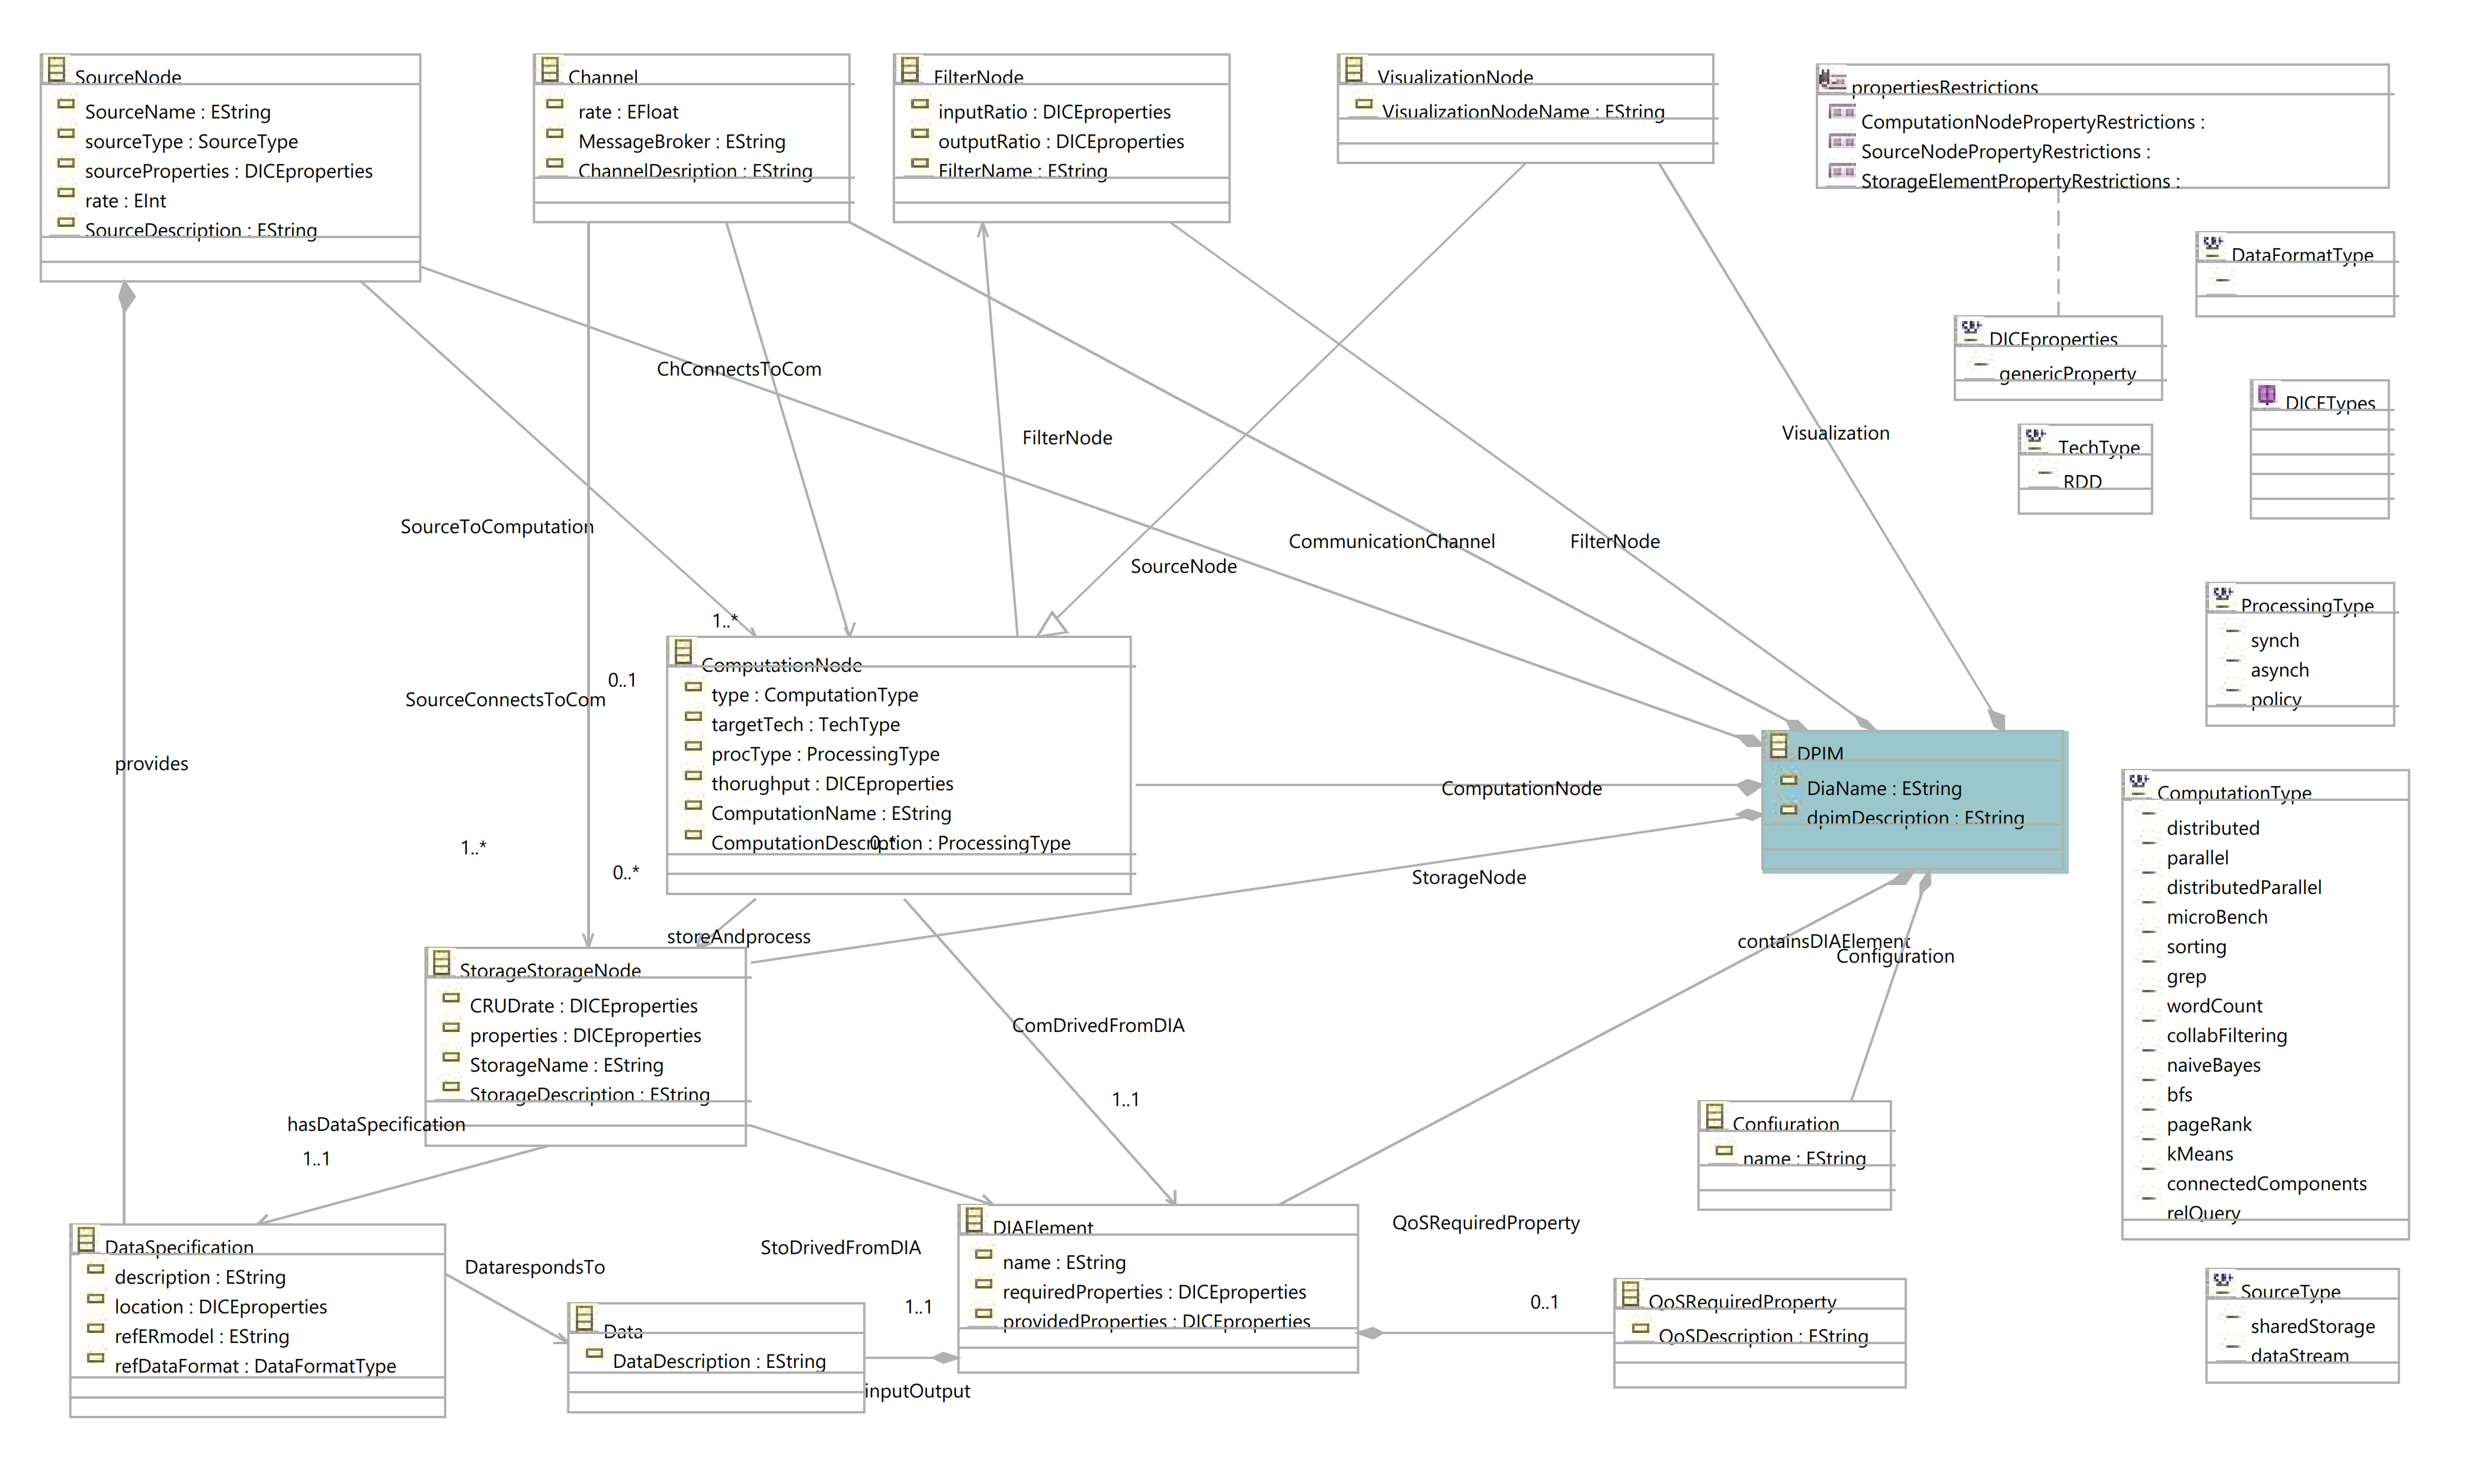
\includegraphics[width=\textwidth]{Images/11.png}
%\caption{\label{fig:metamodel}DICE DPIM metamodel.}
%\end{sidewaysfigure}
%
%\begin{figure}
%\centering
%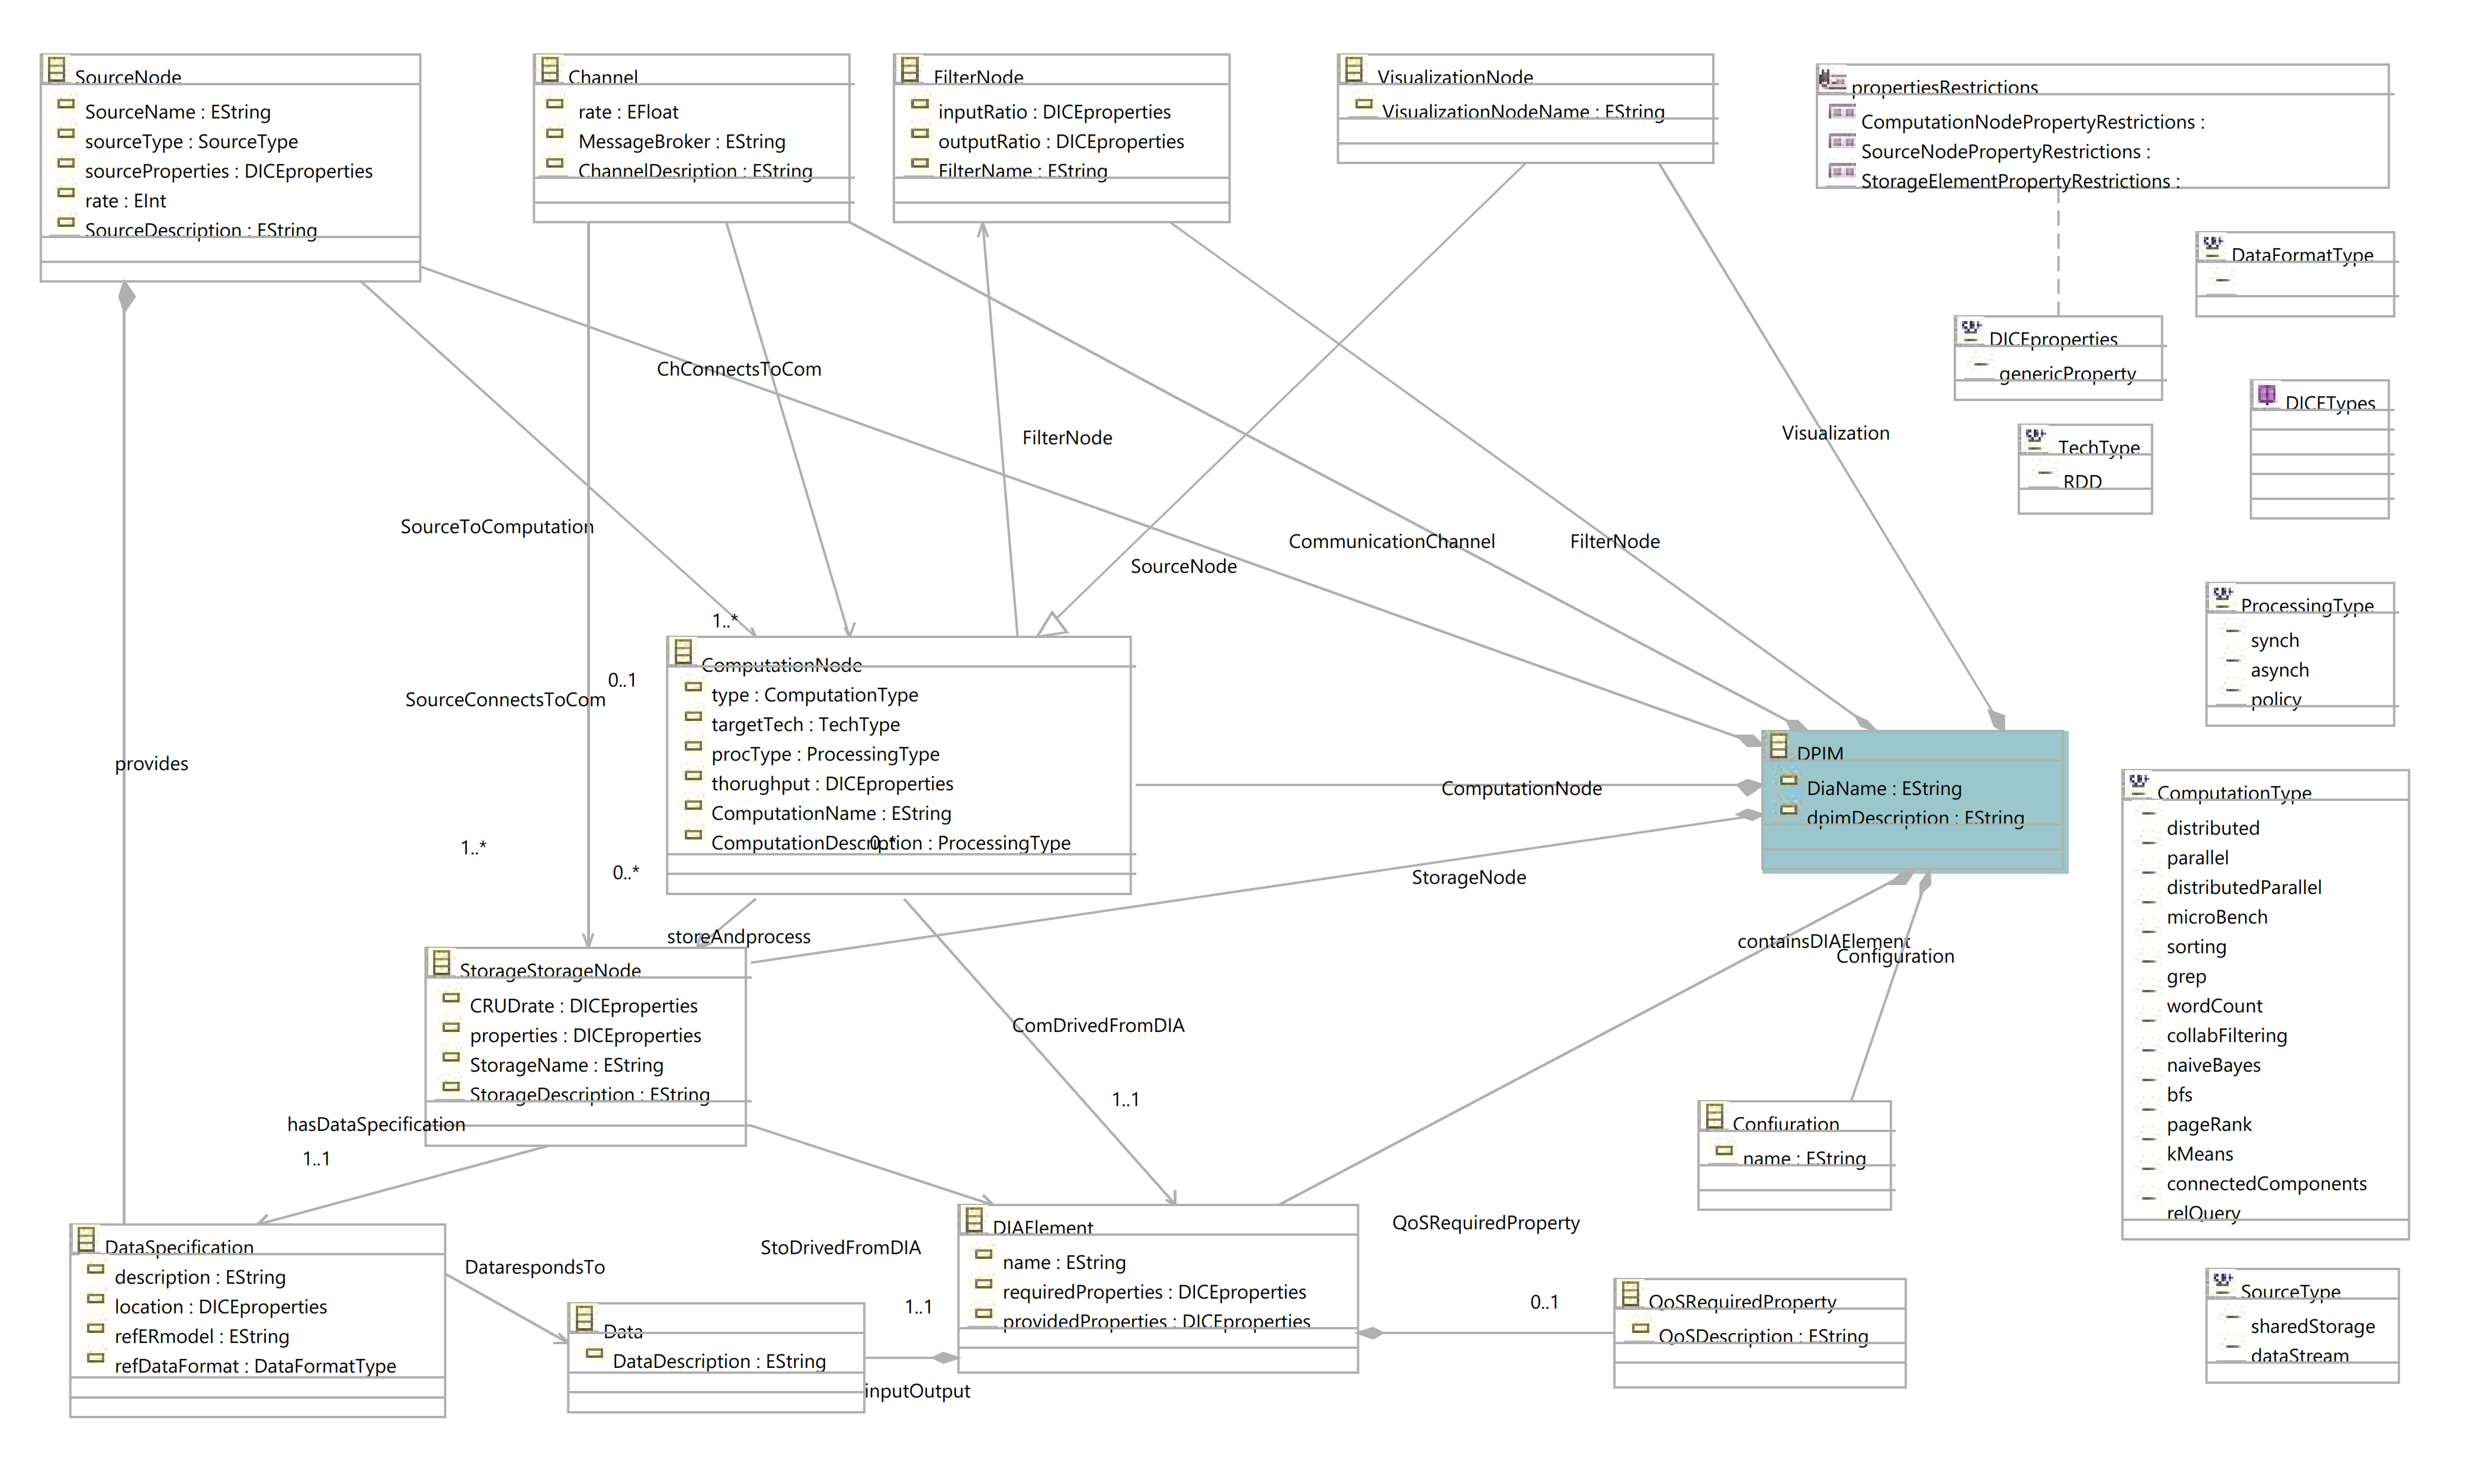
\includegraphics[width=\textwidth]{Images/11.png}
%\caption{\label{fig:metamodel2}DICE DPIM metamodel in portrait form.}
%\end{figure}

%Here is the command to refer to another element (section, figure, table, ...) in the document: \emph{As discussed in Section~\ref{sect:overview} and as shown in Figure~\ref{fig:metamodel}, ...}. Here is how to introduce a bibliographic citation~\cite{DAM}. Bibliographic references should be included in a \texttt{.bib} file. 
%
%Table generation is a bit complicated in Latex. You will soon become proficient, but to start you can rely on tools or external services. See for instance this \href{https://www.tablesgenerator.com}{https://www.tablesgenerator.com}. 


\subsection{Product Perspective}
Here we include scenarios and further details on the shared phenomena and a domain model (class diagrams and statecharts)


\begin{itemize}
\item
main objective of this system is to serve as an interface (intermediary?) between the farmers, agronomists, and policy makers. 
\item
intention is that this system will incorporate data-driven [blank] and include community focused [blank]? 
\item
this system will bridge the gap across these stakeholders with the goal for the telengana to to produce more effective and data-driven policies.
\item
since this is a big problem, with many involved people, people geographically spread out, etc this system provides an interface to that data can be shared and effectively used across users. 
\item
strengthen the cohesiveness of the policies generated and informed by data provided by users
\end{itemize}


\subsection{Product Functions}
Here we include the most important requirements
\par
Maybe add another table here?

% Let's format the requirements table here in a seperate file. We will very likely modify the requirements later on so saving it in a seperate file might make it easier to: 1) see where we need to make modifications and 2) identify formatting errors.
\begin{center}
\begin{longtable}{|c|>{\raggedright\arraybackslash}m{15cm}|}

    \hline
    \multicolumn{2}{|c|}{Begin}\\\hline
    \textbf{ID} & \textbf{Requirement}\\\hline
    \endfirsthead
    
    \hline
    \multicolumn{2}{|c|}{Cont.}\\\hline
    \textbf{ID} & \textbf{Requirement}\\\hline
    \endhead 
 
 
R1	& The system must allow the farmer to set the production types of their fields.\\\hline
R2	& The system must allow the farmer to set the position of their fields manually.\\\hline
R3	& The system must allow the farmer to set the position of their fields through their devices' GPS.\\\hline
R4	& The system must keep track of the data about farmers.\\\hline
R5	& The system must provide an interface to visualize data.\\\hline
R6	& The system must be able to analyze data and show statistics.\\\hline
R7	& The system must enable farmers to modify their production type.\\\hline
R8	& The system must enable farmers to report issues they may face. \\\hline
R9	& The system must allow the farmer to report production data at a frequency chosen by the farmer. \\\hline
R10	& The system must retrieve the weather forecast data from the data that the Telengana government collects.\\\hline
R11	& The system must show updated weather forecast data at most 5 minutes from which the data has been published by the Telengana government.\\\hline
R12	& The system must provide weather data that forecasts at least 3 days ahead.\\\hline
R13	& The system must allow agronomists to access weather forecast data specific to their responsible area.\\\hline
R14	& The system must allow farmers to access weather forecast data based on their GPS location or from the location of their farm on record.\\\hline
R15	& The system must provide an interface for farmers to request help and suggestions from other farmers.\\\hline
R16	& The system must provide an interface for farmers to receive help requests and receive suggestions sent to them from other farmers.\\\hline
R17	& The system must provide an interface for farmers to provide suggestions to other farmers.\\\hline
R18	& The system must provide an interface for farmers to respond to help requests sent to them from other farmers.\\\hline
R19	& The system must provide an interface for farmers to request help and suggestions from other agronomists.\\\hline
R20	& The system must provide an interface for agronomists to receive help requests sent to them from other farmers.\\\hline
R21	& The system must provide an interface for agronomists to respond to help requests sent to them from other farmers.\\\hline
R22	& The system must provide an interface for agronomists to provide suggestions to other farmers.\\\hline
R23	& The system must provide a forum interface.\\\hline
R24	& The system must allow the farmer to create discussion forums.\\\hline
R25	& The system must allow farmers to view all posts in the discussion forum.\\\hline
R26	& The system must allow farmers to post replies in the discussion forum.\\\hline
R27	& The system must keep track of all the forum discussion.\\\hline
R28	& The system must allow agronomists to specify their responsible geographic area.\\\hline
R29	& The system must allow agronomists to modify their responsible geographic area.\\\hline 
R30	& The system must allow agronomist to view the list of all farmers in their area. \\\hline
R31	& The system must provide an evaluation of farmers such that the evaluation reflects the quality and quantity of their crop production.\\\hline
R32	& The system must enable agronomists to access farmer evaluations from their specific area.\\\hline
R33	& The system updates farmers' evaluation when new data is available.\\\hline % (ie, new farmer event entries or after an agronomist visit, etc)
R34	& The system must provide an interface for daily plans.\\\hline
R35	& The system must recommend which farmers should be included in the agronomist's daily plan.\\\hline
R36	& The system must generate recommendations such that farmers are visited by their respective agronomists at least twice a year.\\\hline
R37	& The system must generate recommendations such that farmers with low evaluation are visited more often than twice a year.\\\hline
R38	& The system must allow agronomist to view the list of all farms to visit on a specific day.\\\hline
R39	& The system must allow agronomists to modify which farmers they visit in their plan.\\\hline
R40	& The system must allow agronomists to specify and modify the duration of the visits in their plan.\\\hline
R41	& The system must maintain a record of farmers who have been visited by their respective agronomists.\\\hline
R42	& The system must allow agronomists to modify the daily plan at the end of the day.\\\hline
R43	& The system must allow agronomists to confirm that the daily plan was executed that the end of that day.\\\hline
R44	& The system must not allow anymore modifications to the plan after the plan is confirmed by the agronomist.\\\hline
R45	& The system must only generate a new plan for a new day after the plan from the preceding day was confirmed by the agronomist.\\\hline
R46	& The system must allow Telengana’s policy makers to view the list of all farmers.\\\hline
R47	& The system must allow Telengana’s policy makers to view the performance and evaluation of the farmers.\\\hline
R48	& The system must allow Telengana’s policy makers to view the ranking of the farmers.\\\hline
R49	& The system must allow Telengana’s policy makers to view well-performing and poor-performing farmers.\\\hline
R50	& The system must allow Telengana’s policy makers to flag the farmers that need to be helped based on their performance.\\\hline
R51	& The system must designate each farmer a measure of support received by agronomists and other well-performing farmers.\\\hline
R52	& The system must allow policy makers to view the history of farmers’ performance/ evaluation.\\\hline
R53	& The system must allow Telengana policy makers to view this measure of support designated to each farmer.\\\hline
\end{longtable}
\end{center}


\subsection{User Characteristics}
\begin{flushleft}
This system expects three different types of users: farmer, agronomist, and policy maker.
\subsubsection{Farmer}
\subsubsection{Agronomist}
\subsubsection{Policy Maker}
A Telengana policy maker is a type of user that intends to use the DREAM system to drive policy decisions. Policy makers are mainly interested in accessing rankings and evaluations of all the farmers in the entire area as well as identifying broader trends in the data such as relating the community-provided support to production outcomes. Since policy makers have a more holistic view of the region, they use the DREAM system to configure metrics that are used to classify "well-performing" and "poor-performing" farmers based on rankings, evaluations, and data.\\
%\begin{itemize}
%\item
%mainly interested in seeing the evaluations generated by the system
%\item 
%may configure the metric to classify “well-performing” and “bad-performing” farmers based on rankings generated by system, evaluations from data, and natural/ climate circumstances specific to the year 
%\item
%will use the results seen on DREAM system to make policy decisions. These policy decisions exists outside of the system but will eventually affect the farmers and their production therefore may have an indirect after-effect on the data later inputted into the system
%\item
%the system should provide sufficient and clear data and analysis to enable telengana policy makers to make clear determinations of the efficacy of their policy decisions. 
%\end{itemize}
%



\end{flushleft}


\subsection{Assumptions, dependencies and constraints}
Here we include domain assumptions


% Assumptions Table
\newcounter{assum_counter}
\setcounter{assum_counter}{1}

\begin{table}
\centering
\caption{\label{tab:addOne{table_counter}}Domain Assumptions.}

\renewcommand{\arraystretch}{1.25}
\begin{tabular}{|l|>{\raggedright\arraybackslash}m{12cm}|} \hline
    \textbf{ID} & \textbf{Domain Assumption}\\\hline
	D\addOne{assum_counter} & Users must have a device connected to internet.\\\hline
	D\addOne{assum_counter} & To access to the system the user must have valid credentials.\\\hline
	D\addOne{assum_counter} & The data about weather forecast, the farmers and their production, the sensors, the agronomist are correct, complete and sent to the application. \\\hline
	D\addOne{assum_counter} & The user has granted permission for GPS, notifications and disk usage.\\\hline
	D\addOne{assum_counter} & Farmers have an existing system to quantify, track, and organize their production yields.\\\hline
	D\addOne{assum_counter} & Users can successfully operate an interactive application.\\\hline
	D\addOne{assum_counter} & Business competition will not influence the farmers' willingness to help.\\\hline
	D\addOne{assum_counter} & Farmers are willing to ask for help from other farmers and/or agronomists.\\\hline
	D\addOne{assum_counter} & Farmers have industry knowledge about fertilizers, crops, etc.\\\hline
	D\addOne{assum_counter} & Farmers are willing to interact with other farmers.\\\hline
	D\addOne{assum_counter} & Farmers can recognize issues and production abnormalities.\\\hline
	D\addOne{assum_counter} & Agronomists are assigned an area by their superiors.\\\hline
	D\addOne{assum_counter} & Agronomists can effectively manage an area assigned to them (ie, the agronomist is not overworked).\\\hline
	D\addOne{assum_counter} & Agronomists are experts in their field.\\\hline
	D\addOne{assum_counter} & Agronomists will be effective in addressing issues farmers face.\\\hline
	D\addOne{assum_counter} & Agronomists have access to an internet connection.\\\hline
	D\addOne{assum_counter} & Agronomists can successfully operate an interactive application.\\\hline
	D\addOne{assum_counter} & Weather forecast data is available.\\\hline
	D\addOne{assum_counter} & Weather forecast data is accurate.\\\hline
	D\addOne{assum_counter} & Farmers are not interested in meteorological changes that occur in less than 5 minutes.\\\hline
	D\addOne{assum_counter} & Agronomists are effective in determine performance based on various data points.\\\hline
	D\addOne{assum_counter} & Modifications to the daily plan are simple.\\\hline
	D\addOne{assum_counter} & confirmed plans actually happened /..... [better worded].\\\hline
	D\addOne{assum_counter} & Policy makers want to see the success of farmers in the form of production yields and crop quality.\\\hline
\end{tabular}
\end{table}




%------------------------------------------------------------------------------------------------------------------------------------------------
\clearpage
{\color{Blue}{\section{Specific Requirements}}}
\label{sect:requirements}
Organize this section according to the rules defined in the project description. 
\subsection{External Interface Requirements}
\subsubsection{User Interfaces}
\subsubsection{Software Interfaces}
\subsubsection{Communication Interfaces}
\subsection{Functional Requirements}
Definition of use case diagrams, use cases and associated sequence/activity diagrams, and mapping on requirements

%Use this counter for the scenarios and command \addOne to print and increase at the same time
\newcounter{usecase_counter}
\setcounter{usecase_counter}{1}

% Usecases TEMPLATE
%% Scenario Text
\begin{flushleft}
\textbf{Scenario \addOne{usecase_counter}:} 
\textit{Here enter the scenario story that is associated with this use case. Choose a name for the character, preferably one from New Girl???? [Jess, Winston, Cece, Nick, Schmidt, etc] and describe the scenario with sufficient detail to showcase it's relevancy to the functions of the system.}
\end{flushleft}
%% Use Case Table
\begin{center}
\begin{tabular}{|l|>{\raggedright\arraybackslash}m{12cm}|}

    \hline
    \textbf{Name} & \textit{Name of the Use Case}\\
    \hline
   	\textbf{Actor} & \textit{Farmer, Agronomist, or Policy Maker}\\
    \hline
    \textbf{Entry Conditions} & \textit{Enter the entry conditions required for this use case to be relevant/ applicable}\\
    \hline
    \textbf{Events Flow} & \textit{Enter the flow flow splash splash of events}\\
    \hline
    \textbf{Exit Conditions} & \textit{Enter the circumstances required to exit this use case situation}\\
    \hline
    \textbf{Exceptions} & \textit{Enter and exceptions}\\
    \hline
\end{tabular}
\end{center}
%\input{Files/sequence_diagrams/sequence_diagram_stencil_pic.jpg}

%FARMERS
% Scenario Text
\begin{flushleft}
\textbf{Scenario \addOne{usecase_counter}:} 
Max is a farmer who cultivates some fields near his house in Telangana state. Max has been planting the same plant species over the last few years; he refrains from trying different plants because he is unfamiliar with the cultivation methods. Now, with more children and grandchildren to feed, he would like to change the crop with something more productive. Max learned about the DREAM initiative from a friend and, through the Association of Farmers, he received his credentials to log into the website.
Within minutes of accessing the site, he skimmed through the discussion forums and discovered that there are thousands of small farmers like him with the same doubts and fears. He learned which species are more productive and which fertilizer to use. Now he can feed his entire family and even sell some food to the local market.
\end{flushleft}
% Use Case Table
\begin{center}
\begin{tabular}{|l|>{\raggedright\arraybackslash}m{12cm}|}

    \hline
    \textbf{Name} & \textit{Create a thread in farmers' forum}\\
    \hline
   	\textbf{Actor} & \textit{Farmer}\\
    \hline
    \textbf{Entry Conditions} & \textit{The user uses valid credentials to log into the application}\\
    \hline
    \textbf{Events Flow} & \textit{
    		\begin{enumerate}
    			\item The user opens the forums section
    			\item The user clicks on "Create thread"
    			\item The user writes a valid title and message
    			\item The user clicks on "Publish"
    			\item The user can answer to messages published in his conversation
    		\end{enumerate}
    	}\\
    \hline
    \textbf{Exit Conditions} & \textit{The user closes the forum section or the entire application}\\
    \hline
    \textbf{Exceptions} & \textit{
    		\begin{itemize}
    			\item The server is not available
    		\end{itemize}
    	}\\
    \hline
\end{tabular}
\end{center}
% Scenario Text
\begin{flushleft}
\textbf{Scenario \addOne{usecase_counter}:} 
Caroline has a big farm in Telangana state with 50 hectares of land and different varieties of plants. Last year, during the monsoon season, her fields were flooded, and almost no plants survived. In addition, this summer, the hot temperature killed some other species.
After consulting an expert, she decided to join the DREAM initiative to ask for direct support from agronomists and to obtain some incentives from the central government.
Next year she will plant more resilient crops and take some precautions against flooding.
\end{flushleft}
%\input{Files/sequence_diagrams/sequence2.jpg

% Usecases related to agronomist
% \input{Files/usecases/usecase3.tex}
% \input{Files/usecases/usecase4.tex}

% Usecases related to policy maker
\input{Files/usecases/policy1.tex}
%
%\textbf{EXAMPLE:} if the system determines that precipitation levels are decreasing and enabling a water scarcity crisis, policy makers should be able to see that identify that trend in the system and this can motivate them to enforce policy such as investing in water irrigation technologies that increase efficiency and reduce water waste. Once such policies are in place, telengana policy makers can identify if the new policy mediates the water scarcity problem. 
%\\

% \input{Files/usecases/usecase6.tex}
% .......


\subsection{Performance Requirements}
\subsection{Design Constraints}
\subsubsection{Standards compliance}
\subsubsection{Hardware limitations}
\subsubsection{Any other constraints}
\subsection{Software System Attributes}
\subsubsection{Reliability}
\subsubsection{Availability}
\subsubsection{Security}
\subsubsection{Maintainability}
\subsubsection{Portability}

%------------------------------------------------------------------------------------------------------------------------------------------------
\clearpage
{\color{Blue}{\section{Formal Analysis Using Alloy}}}
\label{sect:alloy}
\begin{flushleft}
Organize this section according to the rules defined in the project description. 


This section should include a brief presentation of the main objectives driving the formal modeling activity, as well as a description of the model itself, what can be proved with it, and why what is proved is important given the problem at hand. To show the soundness and correctness of the model, this section can show some worlds obtained by running it, and/or the results of the checks performed on meaningful assertions.

\end{flushleft}


\lstinputlisting[language=alloy]{../AlloyCode/DREAMS.als}

%------------------------------------------------------------------------------------------------------------------------------------------------
\clearpage
{\color{Blue}{\section{Effort Spent}}}
\label{sect:effort}
%Provide here information about how much effort each group member spent in working at this document. We would appreciate details here.

\begin{table}[!ht]
\centering
\begin{tabular}{|p{0.35\textwidth}|p{0.15\textwidth}|p{0.15\textwidth}|}
\hline
\multicolumn{3}{|c|}{\textbf{Gabriele Marra}}            \\ \hline
\textbf{Task}                   & \textbf{Time} & \textbf{Date} \\ \hline

First Meeting				&		1.0h	   &	2021/10/20 \\ \hline
Goals and phenomena			&		1.0h	   & 	2021/11/20 \\ \hline
Goals meeting					&		1.5h	   &	2021/11/21 \\ \hline
Requirements		&		1.0h	   &	2020/11/23 \\ \hline
Working on requirements and domain assumption			&		3.0h	   &	2021/11/24 \\ \hline
Requirements  meeting		&		3.5h	   &	2021/11/25 \\ \hline
Scenario and use cases		&		2.5h    &   	2021/11/29 \\ \hline
Scenario and use cases meeting		&		3.0h	   & 	2021/11/30 \\ \hline
Use cases meeting		&		1.5h	   & 	2021/12/01 \\ \hline
Product function and user description		&		1.5h	   & 	2021/12/03 \\ \hline
Alloy meeting				&		2.0h     &	2021/12/08 \\ \hline
Sequence diagrams			&		1.5h	  &	2021/12/09 \\ \hline
Sequence diagrams meeting				&		3.0h	   & 	2021/12/09 \\ \hline
Alloy working				&		3.0h	  &    2021/12/11 \\ \hline 
Alloy working				&		2.5h	  &    2021/12/13 \\ \hline 
Alloy working				&		2.5h	  &    2021/12/14 \\ \hline 
Alloy refinement and testing		&		3.0h	  &    2021/12/16 \\ \hline
Design mockup			&		1.5h	  &    2021/12/17 \\ \hline 
Alloy cleaning and description		&		3.5h	  &    2021/12/18 \\ \hline
RASD check				&		3.0h   &	2021/12/20 \\ \hline
RASD finishing				&		4.0h	  &    2021/12/21  \\ \hline
RASD final review			&		3.0h	  &    2021/12/22  \\ \hline
\textbf{Total}                  		&  \textbf{52 h}   & \\ \hline
\end{tabular}
\end{table}


\begin{table}[!ht]
\centering
\begin{tabular}{|p{0.35\textwidth}|p{0.15\textwidth}|p{0.15\textwidth}|}
\hline
\multicolumn{3}{|c|}{\textbf{Matteo Miceli}}            \\ \hline
\textbf{Task}                   & \textbf{Time} & \textbf{Date} \\ \hline

First Meeting				&		1.0h	   &	2021/10/20 \\ \hline
Goals and phenomena			&		1.0h	   & 	2021/11/20 \\ \hline
Goals meeting					&		1.5h	   &	2021/11/21 \\ \hline
Requirements		&		1.0h	   &	2020/11/23 \\ \hline
Working on requirements and domain assumption			&		3.0h	   &	2021/11/24 \\ \hline
Requirements  meeting		&		3.5h	   &	2021/11/25 \\ \hline
Scenario and use cases		&		2.5h    &   	2021/11/29 \\ \hline
Scenario and use cases meeting		&		3.0h	   & 	2021/11/30 \\ \hline
Use cases meeting		&		1.5h	   & 	2021/12/01 \\ \hline
Product function and user description		&		1.5h	   & 	2021/12/03 \\ \hline
Alloy meeting				&		2.0h     &	2021/12/08 \\ \hline
Sequence diagrams			&	 2.0h	  &	2021/12/08 \\ \hline
Sequence diagrams meeting				&		3.0h	   & 	2021/12/09 \\ \hline
UML and sequence diagrams meeting				&		2.0h	   & 	2021/12/10 \\ \hline
Sequence diagrams			&		2.0h	  &	2021/12/12 \\ \hline
Diagrams meeting				&		1.0h	   & 	2021/12/14 \\ \hline
Alloy working				&		2.0h	  &    2021/12/16 \\ \hline 
Design mockup			&		1.5h	  &    2021/12/17 \\ \hline 
Goal mapping	&		3.0h	  &    2021/12/17  \\ \hline
Goal mapping	&		3.0h	  &    2021/12/18  \\ \hline
RASD check				&		1.0h   &	2021/12/20 \\ \hline
RASD finishing				&		1.0h	  &    2021/12/21  \\ \hline
RASD final review			&		2.0h	  &    2021/12/22  \\ \hline
\textbf{Total}                  		&  \textbf{45 h}   & \\ \hline
\end{tabular}
\end{table}


\begin{table}[!ht]
\centering
\begin{tabular}{|p{0.35\textwidth}|p{0.15\textwidth}|p{0.15\textwidth}|}
\hline
\multicolumn{3}{|c|}{\textbf{Destiny Mora}}            \\ \hline
\textbf{Task}                   & \textbf{Time} & \textbf{Date} \\ \hline

First Meeting				&		1.0h	   &	2021/10/20 \\ \hline
Goals and phenomena			&		1.0h	   & 	2021/11/20 \\ \hline
Goals meeting					&		1.5h	   &	2021/11/21 \\ \hline
Requirements		&		1.0h	   &	2020/11/23 \\ \hline
Working on requirements and domain assumption			&		3.0h	   &	2021/11/24 \\ \hline
Requirements  meeting		&		3.5h	   &	2021/11/25 \\ \hline
Scenario and use cases		&		2.5h    &   	2021/11/29 \\ \hline
Scenario and use cases meeting     	&		3.0h	   & 	2021/11/30 \\ \hline
Use cases meeting		&		1.5h	   & 	2021/12/01 \\ \hline
Product function and user description		&		1.5h	   & 	2021/12/03 \\ \hline
Alloy meeting				&		2.0h     &	2021/12/08 \\ \hline
Sequence diagrams			&		1.5h	  &	2021/12/09 \\ \hline
Sequence diagrams meeting				&		3.0h	   & 	2021/12/09 \\ \hline
UML and other diagrams				&		2.0h	   & 	2021/12/13 \\ \hline
Diagrams meeting				&		1.0h	   & 	2021/12/14 \\ \hline
Alloy working		&		1.0h	  &    2021/12/16 \\ \hline
Alloy refinement and testing		&		2.5h	  &    2021/12/16 \\ \hline
Design mockup			&		4.0h	  &    2021/12/17 \\ \hline 
Section 1 and 2 writing 			&		3.0h	  &    2021/12/19 \\ \hline 
Section 3 writing 			&		2.0h	  &    2021/12/20 \\ \hline 
RASD check				&		1.5h   &	2021/12/20 \\ \hline
RASD finishing				&		3.0h	  &    2021/12/21  \\ \hline
RASD final review			&		2.0h	  &    2021/12/22  \\ \hline
\textbf{Total}                  		&  \textbf{48 h}   & \\ \hline
\end{tabular}
\end{table}




%------------------------------------------------------------------------------------------------------------------------------------------------
\clearpage
\addcontentsline{toc}{section}{References}
\bibliographystyle{plain}
\bibliography{main}
%------------------------------------------------------------------------------------------------------------------------------------------------




\end{document}
